%\section{Introduction}
\begin{itemize}
    \item short introduction, no more than the first page, just to set this section up
\end{itemize}

\section{Automatic Speech Recognition in DSP}
\begin{itemize}
    %\item Working title, not married to it
    \item sets up pre-deep learning ASR techniques
    %\item here we can cover very early ASR
    \item The FFT, spectrograms and mel-spectrograms
    \item Spectrograms, EMGs and other tools used in linguistics.
    \item HMMs
    \begin{itemize}
        \item for HMMs we should set up best pre-deep learning WER
        \item we could also set up the idea of the limited datasets available
    \end{itemize}
\end{itemize}



\subsection{The Fourier Transform and Mel-Spectrograms}
\begin{itemize}
    \item Cover the maths of the FFT
    \item Introduce the spectrogram
    \item Cover the mel-spectrogram and the linguistic theory behind it
    %\item I can put a figure of a mel-spectrogram here 
\end{itemize}

\subsection{Engineering and Linguistics}
\begin{itemize}
    \item How the spectrogram changed linguistics
    \item Measuring F1 through the FFT and the cepstrum spectrum
    \item Manners of articulation
    \item Graphing formants and mapping them to phonemes
    \item I should also cover diphthongs directly and their relationship to MoA, formants and phonemes
    \item Maybe a mel-spectrogram figure here for a specific phoneme, with labels to the formants and MoA
\end{itemize}

\subsection{Hidden Markov Models}\naominote{I do not need a whole section on HMMs!}
\begin{itemize}
    \item HMMs (and their relationship with mel-spectrograms)
    \item Cover the maths of HMMs and their linguistic theory
    \item Training an HMM model
    \item Datasets prior to 2015: WSJ, TIMIT (Irish TIMIT? for the shoutout), switchboard
    \item It may be worth mentioning the size in hours of all of these datasets and how a lot of accents and languages were quite limited in the data.
    \item Cover HMM best WERs on pre 2015 datasets
        \begin{itemize}
            \item for HMMs we should set up best pre-deep learning WER
            \item we could also set up the idea of the limited datsets available
        \end{itemize}
    %\item LibriSpeech was 2015, deepspeech was 2014 and used 5000 hours of their own unbpublished data deepspeech 2 was 2016
\end{itemize}

\hl{Maybe I could cover other machine learning techniques here, like k-means for later BERT discussion}\thoughts{The issue here is the only ML technique that is relevant is k-means and that is only relevant to HuBERT pretraining, which I don't use in any of my experiments.}

%\hl{I could possibly put a linguistics section here covering some of the things pasad et al. find in wav2vec plus MoA}


\section{Deep Neural Networks for ASR}
\begin{itemize}
    %\item Alternative Title "Deep Neural Networks for ASR"
    \item DNNs for other applications like image recognition
    \item Deepspeech and RNNs
    \item Highlight the large dataset size for deepspeech
    \item This then can set up the dataset size race
    \item CNNs and early ASR models
    \item Quartznet \cite{quartznet}
    \item talk about all of the different language variations for quartznet
    \item Adapters and the issue of multi-domain training
    \item the catastrophic forgetting principal
    \item We can set up MLS and maybe common voice for the next section
\end{itemize}

\subsection{Early Neural Networks}
\begin{itemize}
    \item Quick overview of original 60s paper and a few papers over the years
    \item descriptions of important concepts
    \begin{itemize}
        \item backpropagation (hinton, 1986) 
        \item loss objectives: MSE, cross-entropy, KL-divergence 
        \item random initialisation
        %\item \hl{these concepts so far are all directly relevant}
    \end{itemize}
\end{itemize}



\subsection{Recurrent and Convolutional Networks}
\begin{itemize}
    \item CNNs 1980-1997, 1989 on handwriting task 
    \begin{itemize}
        \item could change this around:
        \item CNNs were used for handwriting recognition as was CTC Loss, so it might flow better near CTC
    \end{itemize}
    \item RNNs were invented sometime between 1982-1990
    \item LSTMs 1997-2005, with 2005 being bi-directional as used from then on
    \begin{itemize}
        \item relevant as they are the precursor to transformers
        %\item not sure if any models I cover use them, but it's probably still important to cover them since they relate to transformers
        \item There are also some RNN and LSTM models in the pruning papers, so probably worth covering
    \end{itemize}
    \item autoencoder 1989-1990
\end{itemize}

\subsection{Connectionist Temporal Classification Loss}
\begin{itemize}
    %\item alternative section header: handwriting recognition; Connectionist Temporal Classification Loss;
    %\item OR this subsection could briefly go over early image recognition and then handwriting recognition
    %\item that might introduce the concept of CTC well...
    \item levenstein distance for WER and CER
    \item CTC loss - 2006 handwriting using LSTM and RNN architecture
    \item Introduce deepspeech and it's use of CTC
    %\item It's difficult to be sure where to put CTC, since it is a loss function and could be explained alongside them
    %\item for now, this works
    %\item Deepspeech by baidu was the first DNN to use CTC for ASR, so does CTC needs its own section?
    %\item I could add some nice figures for CTC and it is important
\end{itemize}



\subsection{Deep Neural Networks}
\begin{itemize}   
    \item Brief description of the rise of GPUs, big data and Deep Networks
    \item Brief description of DNNs for image recognition and the seminal papers using GPUs
    \item description of deepspeech \cite{citationrequired}
    \item deepseech and matching (2014) SOTA HMM WERs \cite{citationrequired}
    \item deepspeech 2 beating HMM WERs \cite{amodei16_deepeech2}
    \item Overview of various common techniques:
    \begin{itemize}
        \item mel-spectrograms as inputs
        \item dropout - 2012
        \item data augmentation - AlexNet 2012, SpecAugment 2019
        \item batch normalisation - 2015
    \end{itemize}
    \item Comment on the size of the datasets used for deepspeech and the fact they were not open-sourced
\end{itemize}


\subsection{Big Data}
\begin{itemize}
    \item \colorbox{yellow}{\textcolor{red}{Medium to easy difficulty to write}}
    \item \colorbox{purple}{\textcolor{white}{Covered across multiple sources}}
    \item reference earlier speech datasets like WSJ
    \item The issue of small open-source datasets for DNNs
    \item Librispeech \cite{librispeech} and it's impact - \textasciitilde 1000h
    \item Common Voice \cite{ardila-etal-2020-common} and open sourcing
    \item AISHELL-2 (2018) [Mandarin] \cite{needtoadd} and multilingual data outside of English
    \item The issue of bias in many of these datasets
    \item Diverse datasets with comments on their pushback against bias and the desire in academia for more diverse datasets
    \begin{itemize}
        \item AAVE 2020 \cite{chang2024self}
        \item Datatang 2020 \cite{aesrc2020}
        \item FLEURs 2022 \cite{FLEURS} 
    \end{itemize}
    \item MLS (2020) \cite{MLS},  and the start of the dataset size alms race
    \item Comment on the significance of having Spanish, French, German open source read speech datasets the same size as LibriSpeech (=>1k hours each)
    \item I should spend some time with MLS. I may need to comment on specifics, such as a lot of the Spanish book being English books translated to Spanish.
    \item Then comment on the ridiculous size of MLS English (44k hours) and how bias was still a problem
    \item Include a list of the big big datasets including comments
    \begin{itemize}
        \item voxpopuli (400k) \cite{wang-etal-2021-voxpopuli}
        \item librilight (60k hours) \cite{librilight}
        \item There are more, but since I don't use any of these maybe don't spend too much time with this.
    \end{itemize}
    \item This section needs to cover all relevant datasets
    \begin{itemize}
        \item or do I have a separate section later on for just the directly relevant ones for my experiments?
    \end{itemize}
    \item I could also have some comments at the end on much more recent datasets. Such as recent large Irish, Gaelic and Hindi datasets that show that the desire for more diverse data has been a big change in the last \textasciitilde 5 years
    \item \textbf{Now we have the big data we set up the model size race.}
\end{itemize}

\subsection{CNNs for speech}
\begin{itemize}
    \item \colorbox{yellow}{\textcolor{red}{Medium difficulty to write}}
    \item \colorbox{purple}{\textcolor{white}{In confirmation report}}
    \item Jasper (as the precurser to QN) architecture \cite{needsjaspercitation}
    \item Quartznet15x5 (2020) architecture \cite{quartznet}
    \begin{itemize}
        \item since this currently isn't in my thesis we don't need quite as much depth
        \item however, this is still a good explanation of CNNs as feature extractors for later wav2vec
    \end{itemize}
    \item feature extraction
    \item Monolingual Quartznets for different languages
    \item catastrophic forgetting
    \item Adapter layers and the issue of multilingual training
    \item Layer freezing and supervised learning layer analysis
    \item Parameters in QN and efficiency of CNNs
    \item \hl{Much of this is interesting and somewhat relevant, but without the actual Quartznet15x5 experiments included, only some of it is directly relevant and completely necessary. I should write this towards the end when I have a better sense for what I want to include.}
\end{itemize}




%%%%%%%%%%%%%%%%%%%%%%%%%%%%%%%%%%%%%%%%%%%%%%%%%%%%%%%%%%%%%%%%%%%%%%%%%%%%%%%%%%%%%%%%%%%%%%%%%%%%
\hl{Original Model analysis section!!!!}

\section{Model Analysis}

While, model compression techniques have not yet revealed the inner workings of multilingual SSL ASR there have been other attempts to deconstruct them. \hl{If I want to talk about supervised learning model analysis it could be a short 1/2 paragraphs here.}

\hl{Copied from previous background sections, needs adapting}

Previous studies show significant difference between the tasks learned on each layer\cite{belinkov2017analyzing} for DeepSpeech2 \cite{amodei2016deep}, a previous supervised ASR model. They also show that different categories of phonemes are learned with higher accuracy at different layers. Choi et al. \cite{choi2024self} have found that SSL ASR speech representations exhibit more phonetic similarity than semantic similarity \cite{choi2024self}. 

\subsection{Layer-wise Analysis of wav2vec 2.0}
In 2021, Pasad et al. \cite{pasad2021layer} analysed the inner workings of wav2vec 2.0. They assess the performance of each layer of wav2vec 2.0 in multiple domains: local acoustic features, phone identity, word identity and word meaning. They use Canonical Correlation Analysis (CCA) as a statistical measure of the relationship between layer embeddings for a window of speech data and another vector. These vectors contain linear projections of each of the test domains. 

\begin{figure}
    
    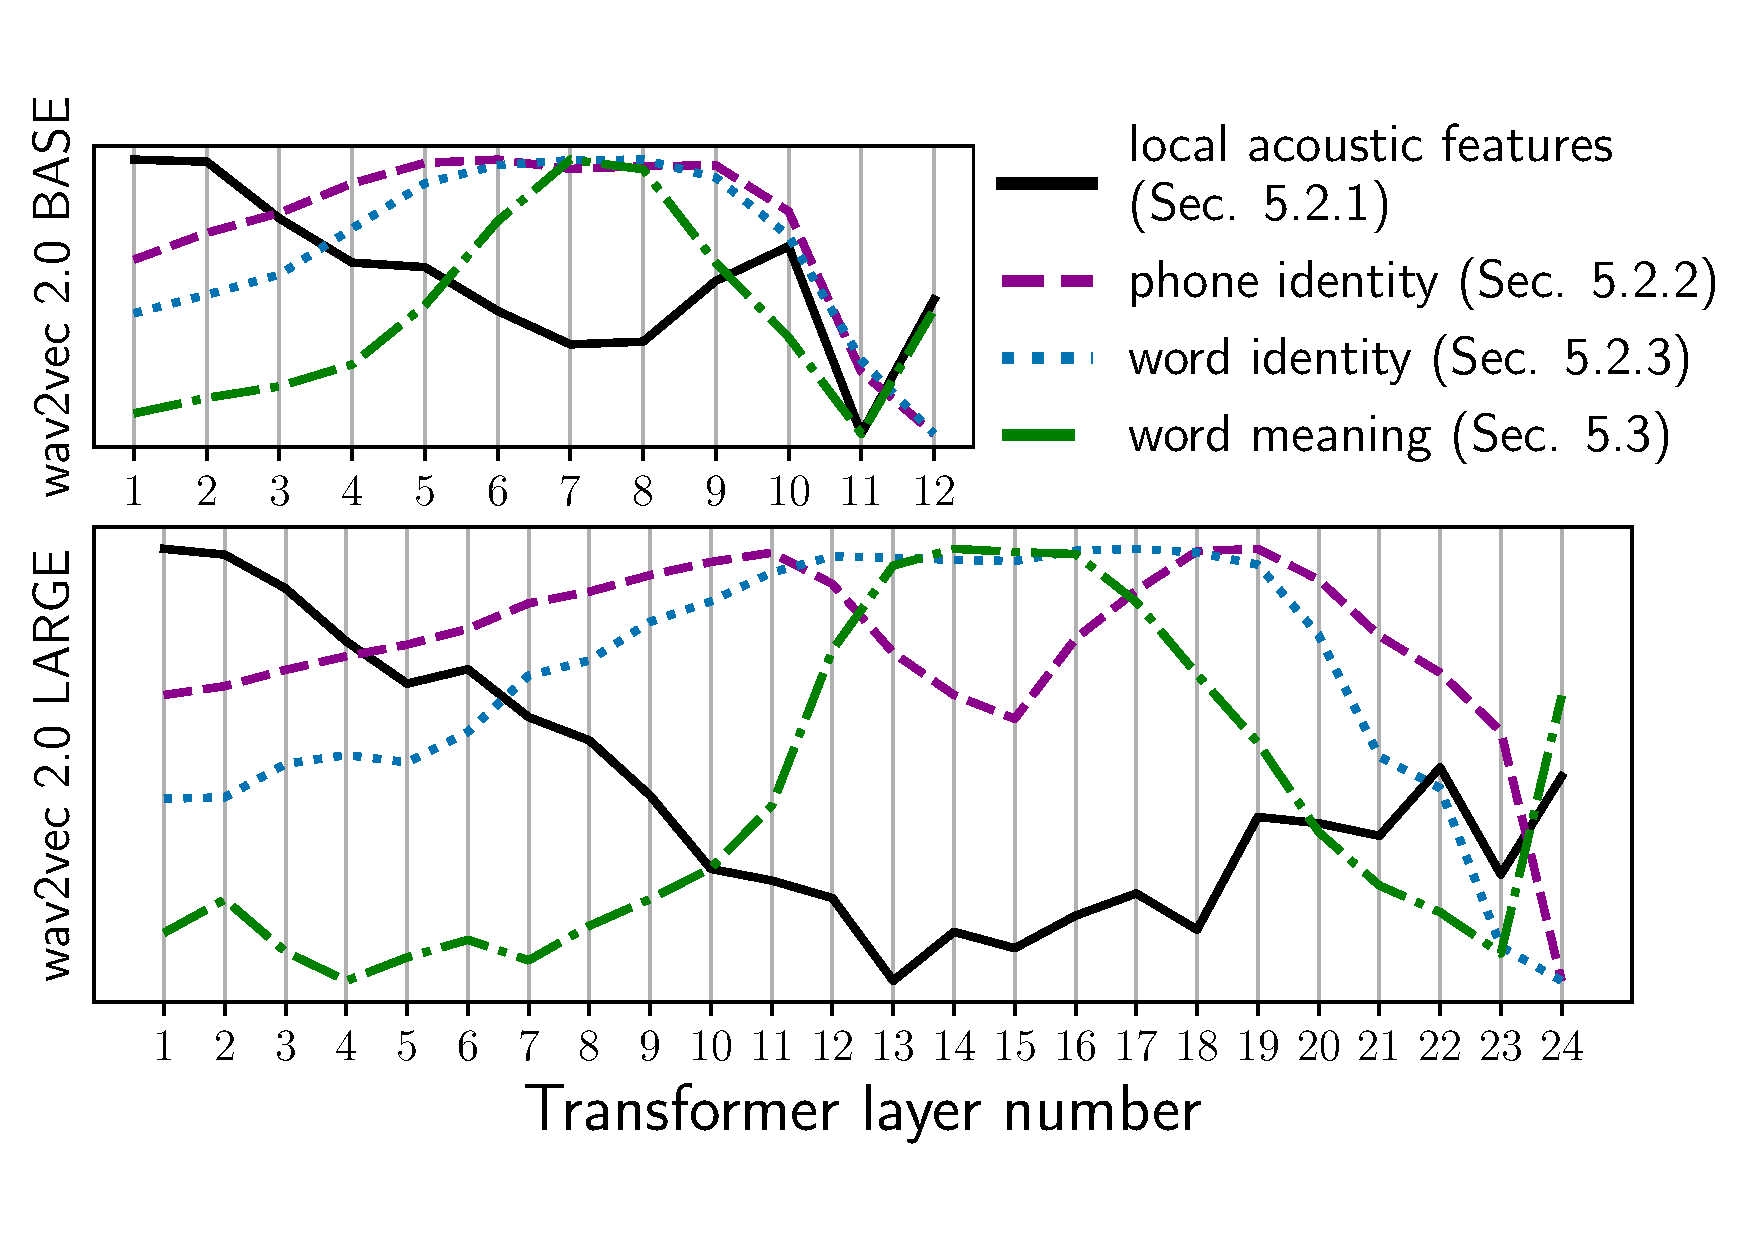
\includegraphics[width=\linewidth,trim={0 40 0 60},clip]{2_chapter2/images/model_analysis/Layer-Wise_Analysis_cropped_graph.pdf}
    \caption{\hl{UPDATE AND MAKE MY OWN} Change this to my label adapted from: \cite{pasad2021layer}}
    \label{lr_fig:language_specific_subnetworks}
\end{figure}

\hl{I use the name encoder a lot, should I change this to conext network for consistency?}

Pasad et al. \cite{pasad2021layer} test two pretrained wav2vec 2.0 models\footnote{\hyperlink{https://github.com/facebookresearch/fairseq/tree/main/examples/wav2vec}{github.com/facebookresearch/fairseq/tree/main/examples/wav2vec}\label{lr_la_fn:w2v2}}: base-LS960, large-VP60k. They first compare model layers when wav2vec 2.0 is finetuned to different amounts if librispeech data: pretrained, 10m, 100h and 960h. They compare each layer to the output of the feature encoder. Both base and large models have high CCA in shallow layers with the feature encoder. CCA then lowers during the middle layers for both models. CCA then rises in deep layers for the pretrained model, but not the finetuned models. 

They label the pretrained CCA pattern as "auto-encoder style behaviour" \cite{pasad2021layer}, due to the rise in CCA in the deep layers.\unexplained{auto-encoder} This behaviour may be an artefact of the contrastive loss function. It teaches the context network to learn codebook entries with high similarity to the feature encoder output. It appears that only the deepest layers of wav2vec 2.0 learn task-dependent weights. This is shown by the finetuned models exhibiting less of the autoencoder behaviour. The more data that is included in finetuning, the lower the CCA is in deep layers. The finetuning loss function is CTC Loss, so the learning objective is character labels. The finetuned deep layers reflect this change in learning objective.

This is further confirmed when comparing hidden states from the feature encoder and the context network to mel-spectrograms. They show that the final layer of the feature encoder shows the highest similarity to the bins of a mel-spectrogram. Similarity is highest in the shallow layers of the context network and decreases for middle and deep layers. Latent speech representations are therefore shown to resemble the linguistic features highlighted in mel-cepstrum spectrums\unexplained{mel-spectrogram, cepstrum spectrums}. This also seems to show that the model is learning broad linguistic information at shallow layers. While deep layers learn more task-specific information.

The context network is not only learning mel-spectrum information, but appears to learn phonemetic and acoustic features. They use the Montreal Forced Aligner (MFA)\unexplained{MFA} to identify phoneme time intervals within each utterance. They collect frames within the phoneme interval and take the average across all frames. They exclude the first and final third of frames within the interval to avoid coarticulation. They also test Acoustically Grounded Word Embeddings (AGWE). Word intervals are found with MFA, then an AGWE is collected by averaging all of the frames within this interval. This gives an acoustic representation of each word.

They find that similarity between hidden states and phonemes is low in shallow layers, highest in middle layers and then reduces again at deep layers. This pattern is true for both pretrained and finetuned models. For the shallow and middle layers, the CCA score is very close between pretrained and finetuned base models. This suggests that the phonetic information is valuable for the finetuning tasks and, so, not forgotten. For deep layers, the finetuned base model has a higher CCA. This shows that phonetic information is more useful for the finetuning objective. This is true for large-VP60k as well. However, it is only the final block that shows a significant difference in CCA between loss objectives. These results suggest the model does not forget the phonetic information learned in pretraining. Phonetic and acoustic information learned in pretraining is transferable to the finetuning task.

A similar pattern can be seen for AGWEs when analysing the pretrained model. However, for the finetuned model, CCA continues to rise in the deepest layers. Here, acoustic representations of full words are valuable since the final task is a transcription. Whereas they are less relevant for the auto-encoder style behaviour of the pretrained model. We know that wav2vec 2.0 codebook entries highly correlate with specific phonemes found in the pretraining data \cite{wav2vec}. So, contrastive loss is encouraging the model to learn phoneme representations. This may be why finetuning does not diverge from already learned phonemes. Word embeddings, however, improve after finetuning, because the pretraining objective does not include fully realised words.

Finally, they assess the similarity between layers from the same models before and after finetuning. They show that for shallow and middle layers, there is high CCA, showing little change in the weight distribution for these layers.\thoughts{Do I use layers or blocks?? They are taking the similarity between the final layer ultimately.} However, the deepest layers, 10-12 for base and 20-24 for large, show reduced CCA. This suggests that shallow and middle layers are learning linguistic information that is transferable between auto-encoder and ASR tasks. The deepest layers learn task-specific information and therefore change the most between training objectives.

Overall, the work of Pasad et al. \cite{pasad2021layer} shows that the information learned during SSL pretraining is transferable to the finetuning task. This illustrates how wav2vec 2.0 is able to achieve low WER with small amounts of finetuning data \cite{wav2vec}. However, due to the contrastive loss in pretraining, the information learned is limited. The pretrained model shows high CCA scores with acoustic and phonetic speech representations. However, for semantic tasks, high similarity is only shown after finetuning with CTC. It is therefore important to understand what acoustic and phonetic information is encoded during the pretraining stage.

\subsection{Approaches to Model Analysis}
\begin{itemize}
    \item Extracted feature comparisons \cite{li2023quantitative}
    \begin{itemize}
        \item dunno how necessary this is to cover, only one small part of the paper is at all relevant
    \end{itemize}
    \item I could use this section to cover stuff like CTC CNN layer analysis for pre wav2vec models
    \begin{itemize}
        \item It would be useful to have this context, since the layers of a supervised model can behave quite differently to an SSL model.
        \item I may have covered it previously though, or it may just not be that relevant
    \end{itemize}
    \item Other different approaches? Pasad has basically become the baseline though, so this may not be necessary
    \item \colorbox{yellow}{\textcolor{red}{Medium difficulty to write}}
    \item \hl{I could also put codebook analysis papers here }
    \item These papers analyse the codebook entries and how that makes the model skewed towards certain domains \cite{wang2025normalization, linke2023self, lee2024balanced}
\end{itemize}

\iffalse
\subsection{Layer Probing}
\begin{itemize}
    \item Phoneme recognition for older models and MFA \cite{mcauliffe2017montreal}
    \item \hl{Do I need to cover MFA in detail or not?}
    \begin{itemize}
        \item ideally yes, so that the examiners understand what it is doing.
    \end{itemize}
    \item Is this a good place to put it, though? Maybe this should be done elsewhere
    \item the paper is from 2017
\end{itemize}
\fi


\subsection{Phonetic Features in Transformers}
\begin{itemize}
    %\item Phoneme recognition for older models and MFA \cite{mcauliffe2017montreal}
    %\item \hl{Do I need to cover MFA in detail or not?}
    %\begin{itemize}
    %   \item ideally yes, so that the examiners understand what it is doing.
    %\end{itemize}
    \item I can mention phoneme annotated data like TIMIT \cite{timit} and the lack of phoneme data available before MFA
    \item not sure exactly where to fit this in, it could equally go after Pasad and maybe even after Cormac's probing stuff since they only use TIMIT. Come back to this later.
    \item I could either move wav2vec + XLSR paper phoneme recognition to here or I could merge this section with the probing stuff.
\end{itemize}

\hl{I need a connecting paragraph here}

\begin{itemize}
    \item I will either briefly list supervised layer analysis papers
    \item OR reference the previous subsection that covers that
    \item Then I will need a short bit on other studies that probe layers (\cite{immer2021probing, schneiderleveraging})
    \item some other relevent papers:
    \begin{itemize}
        \item Nasals in french wav2vec 2.0 \cite{kim2024using}
    \end{itemize}
\end{itemize}

\begin{itemize}
    \item So far, we have covered Pasad's layer analysis, they cover similarity between HSs and various downstream tasks.
    \item The papers we have below cover these techniques: LR probing, MLP probing, CCA similarity, codebook analysis.
    \item The topics they cover: phoneme recognition, MoA recognition, emotion recognition, prosody, AID, LID
    \item I also have the Dan and Hao paper on HuBERT clusters, they use some sort of statistical analysis.
    \item So statr with another statistical analysis paper, maybe dan and hao.
    \item Then probably the Cormac paper to show MoA groups and such
    \item Maybe codebook paper? 
    \item Then the others, listed quickly.
\end{itemize}

The findings of Pasad et al. \cite{pasad2021layer} show that there is significant difference in how self-supervised and supervised speech models learn. With the success of SSL models in speech, understanding exactly how they learned became increasingly important.\thoughts{This intro needs to be rewritten} 

\hl{The into sentence should be something about how pasad didn't find go as deep as articulations}


\begin{figure}
    \centering
    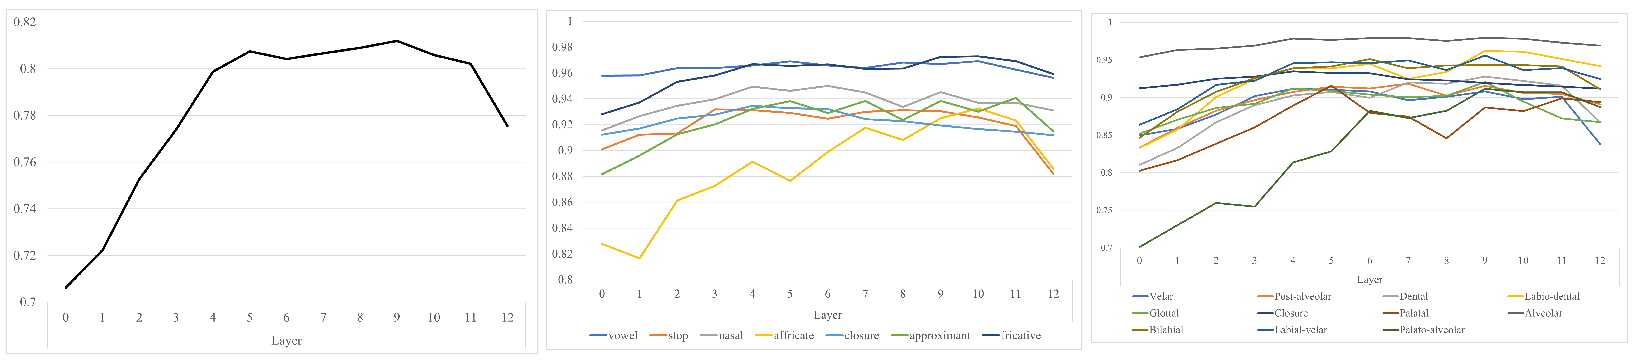
\includegraphics[width=\linewidth]{2_chapter2/images/layer_probing/probe_graphs_single_page_cropped.pdf}
    \caption{\hl{May need updating, graph's are different sizes} Change this to my label adapted from: \cite{english2022domain}}
    \label{lr_fig:layer_probing}
\end{figure}

In 2022, English et al. \cite{english2022domain} collected phoneme accuracy data by training Multi-Layer Perceptron (MLP) probes\unexplained{multi-layer perceptron}\thoughts{an MLP is just a single linear layer, do I need to define this in the early section? Maybe also go through chapter 5 and change releveant probe references to MLP. MLP analsysis/results probe is the item, like the probes perform best on high-resource phonemes.} for phoneme recognition. Each MLP consists of a single linear layer of input size 768, an output of 200, a ReLU\unexplained{ReLU} activation function and a final layer with an output dimension of 1. They use the TIMIT dataset, which has time aligned hand annotated phoneme intervals, to train the probes. Latent phoneme representations are collected from each layer of the wav2vec 2.0 encoder for each window of audio in the TIMIT utterances. For each annotated phoneme, the first and final third of the representations are discarded in order to control for coarticulation. A dataset of each of these phoneme realisations is collected and each probe is then trained for a single task.

First, they recreate the "auto-encoder style" behaviour when measuring the average accuracy across all phonemes at all layers. For manner and place of articulation, they find that layer 7, the 7th transformer block of the conext network, has robust results. Both of these results line up with the findings of Pasad et al. \cite{pasad2021layer}. When measuring manner and place of articulation they find that accuracy varies across classes. Vowels and fricatives have the highest average for MoA classes and alveolar for Place of Articulation (PoA). Although all classes have high accuracy at layer 7, relative to other layers. They then generate confusion matrices and plot both heatmaps and dendrograms to measure phoneme similarity. They find that the phoneme representations at layers 0, 7 and 12 show most similarity to acoustically similar phonemes, such as MoA class. This similarity is most clear at layer 7.

\hl{This is probably enough for this paper, I need to figure out whether I do his other papers here or pasad's other paper. Also, do I need a figure?}

English et al. \cite{english2023discovering} later published follow-up studies that studied how phonetic features (such as voicing, frication and nasal) are encoded in wav2vec 2.0 \cite{wav2vec}. They again probe the model and measure TIMIT phoneme accuracies. They show that frication is well encoded across shallow and middle layers, with a drop in accuracy towards deep layers. Voicing is better encoded in the middle layers, with the highest accuracy at layer 8. Finally, Nasals have consistently high accuracy across all layers. 

Separately from this work, Bosch et al. \cite{ten2023phonemic} also probed wav2vec 2.0 for phonetic features and feature relationships. They found that, generally, probes were an effective approach to analysing SSL models, achieving high accuracy across layers. When analysing phonetic features and phoneme labels they found that middle layers identified individual phonemes clearly. Shallow layers were less able to distinguish between individual phonemes, but could recognise broad phonetic classes (BPCs). BPCs included: plosives, nasals, approximants, fricatives, high vowels, mid vowels, and low vowels. Shallow layers often mislabelled individual phonemes, but were able to distinguish well between BPCs.


Overall, these findings show that SSL models learn broad phonetic features as well as specific phoneme realisations. Building on the findings of Pasad et al. \cite{pasad2021layer, pasad2023comparative} these studies have shown that SSL loss functions teach their models to categorise phoneme realisations into clear phoneme categories. Both comparative loss assigns k-means units to broad phonetic features and creates clusters that represent phonemes.  contrastive loss assigns  


\begin{itemize}
    \item This paper probes a finetuned w2v2 for accent and prosody features \cite{yang2023can}
    \item They use CCA for accent ID task, although it's nto clear if the CCA is between HS and FE output, raw wav, or accent labels
    \item Similar results when comparing pretrained to finetuning (to AID) where later layers have low CCA and final layers raise after FT
    \item Although middle layers are higher in CCA on the pretrained compared to FT
    \item Models FT for ASR have even higher CCA for deep layers
    \item Ok so, CCA is computed with the PHONEME LABEL, so when the L2 speaker gets the phoneme wrong then there may be lower CCA, this is nto necessarily reflective of the model.
    \item a tsne plot shows that for a single phoneme label at layer 9 the phonemes move to clear clusters for each accent. This shows that the model has learned a new mapping for an L2 accent.
    \item They call this clustering "accent specificity"
    \item "In general, we observe a gradual increase of accent specificity in θAID starting from layer 1, and the strongest accent-specificity in layer 9"
    \item They also train linear probes for prosody classification tasks. They find that layer 11 of the pretrained model has the highest accuracy
    \item They theorise that this may be because prosody is closely aligned to semantic information.
\end{itemize}


\begin{itemize}
\iffalse
    \item \hl{I ahven't included Pasad's second paper here }\cite{pasad2023comparative}
    \item \textbf{Extra references:}
    \item I should cover or at least go through this one properly. This is Dan and Hao's 2022 paper on representations in HuBERT \cite{wells2022phonetic}.
    \item Their paper examines HuBERT k-means clusters and how they align with certain phonemes. They analyse phonemes in MoA groups. This is equivalent to analysing the w2v2 codebooks.
    \item \textbf{This 2021 paper MLP} probes multiple models including wav2vec [1.0] and finds that they have high-level phonetic features \cite{ma2021probing}. They also find that MLP probes often perform best compared to other types of probes. They show that thinformation learned by the model is much deeper than a mel-spectrogram.
    \item \textbf{This 2023 interspeech paper} \cite{ten2023phonemic} analyses probing wav2vec 2.0 for phonetic structure. They find that probes generally have high accuracy especially in middle-deep layers even after finetuning,
    \item They then analyse the relationship between the first and second most predicted phonemes. When analysing second most predicted phonemes they find that at early layers vowels cluster closely together often being mistaken for other vowels. At deeper layers their relationship is more "convex". I believe what they mean here is they are more distinguished from one another.
    \item The findings for shallow layers are largely true for all "BPCs" (Broad phonetic classes, basically they mean MoA classes) and for middle-deep layers their findings for vowels are less true for other classes, although still more true than shallow layers.
    \item They claim this means that the model does not need to understand classical linguistic knowledge for the final transcription task.
    \item I would argue that it actually proves the other way, that w2v2 is learning from the top down and by the deeper layers it has clearly identified individual phonemes. Probably why the second most classified phonemes are less related is because it is very good at getting it right so every misclassified phoneme is semi-random. Whereas in early layers it is concentrating on articulation which multiple phonemes share. 
    \item I'm not sure this paper adds a whole lot, other than proving pasad's findings but with probes. I should mention it, but not go into detail.
\fi
    \item Could look at this one \cite{sicherman2023analysingdiscrete} They seem to analyse HS with statistical methods to show they line up with phonemes and categories.
    \item \textbf{This 2023 paper} has an interesting breakdown of entropy in the w2v2 and XLS-R codebooks showing that vowels have more entropy, especially in XLS-R. This may show that not only is the w2v2 family better at vowels but also multilingual data requires more codebook entries to fill all of the different realisations. Unfortunately it is not a multilingual study \cite{abdullah2023information}
    \begin{itemize}
        \item They use information theory to analyse entropy in the w2v2 and xlsr codebooks
        \item They collect windows of phonemes by running them through the quantiser and collecting quantised latents for each phonemem.
        \item They measure the entropy by seeing how much disversity of representations there are for a phoneme. i.e. if a phoneme only has one quantised realisation its entropy is low and if it has many it is high, the most being the total number of entries across the codebooks.
        \item They claim that this similar to the purity metric for hubert
        \item for TIMIT w2v2 has higher entropy than XLSR-53, 56.6\% of entries have a "non zero count" (i.e. are selected 1 or mroe times) whereas it is ony 24.2\% for XLSR-53
        \item For both models vowels are more entropic than consonants
        \item Nasals are the most entropic, while affricates are the least (affricates also only have 2 phonemes)
        \item Voiced fricatives are more entropic than unvoiced
        \item They find that phonemes that share certain representations are gernally driven by articulation class (This is nto well worded by me reread before writing about it)
        \item They claim that codebook entries are sub-phoneme events rather than realised phonemes, similar to Dan Well's paper for HuBERT.
    \end{itemize}
    \item \hl{THIS IS SUCH AN OPEN GOAL!!! UGHHH}
    \item This paper is one to read \cite{nocitation}, they analyse the representations of XLS-R pretrained vs a FT version for LID. There are some nice lookign graphs in this, but I don't have time to read it. \hl{not read yet!}
\end{itemize}

\hl{There are multiple 2022-2024 papers cormac cites that might be relevent to me, I should read them.}

\hl{There are also a lot of good pre-2020 pre-SSL layer analysis references in many of these papers.}


\subsection{Phonetic Features in SSL}
\begin{itemize}
    \item Ask the question: What amount of detail are transformers learning and why?
    \item Start with Dan's HuBERT MoA stuff
    \item Briefly cover cormac's MoA stuff and then include the co-occurrence and coarticulation stuff. That way we have pointed out the level of detail they have learned. This could also go above Dan's stuff actually.
    \item With dan's stuff we have covered the level of detail in the HUBERT loss function so we want to analyse how contrastive loss may be biasing wav2vec 2.0
    \item Do we want to callback to the previous section here or do we want to move it entirely?
    \item The paper on codebook representations would go here.
    \item We then need a more opinion-based discussion on what this means and why these things need to be analysed. 
    \item Such as why does XLSR have less pure entries?
    \item Are the entries multi or monolingual
    \item Dan hints at different accents having an effect on units, but doesn't go into detail. Multilingual is noted as a future work project.
    \item Although broad features are learned, are they effectively shared and if so/if not why?
    \item How does the data source affect this?
    \item Possibly this discussion would require it's own short section and/or written after everything else.
\end{itemize}

\hl{Need to connect these sections.}


They also study the co-occurrence of phonetic features. Exclusive features that can not co-occur, such as articulations, are often considered mutually exclusive by wav2vec 2.0. However, features such as frication and voicing often co-occur. Voicing is not mutually exclusive with any articulation, and wav2vec 2.0 seems to have learned this. Feature co-occurances are shown in their later paper \cite{english2024searching} to follow similar patterns to phonemeic accociations found in linguistics studies \cite{sagey1986representation}. These associations were found inwav2vec 2.0 by probing layer 9 of the context network. In their final paper on probing wav2vec 2.0 \cite{wav2vec}, English et al. \cite{english2024following} also show that wav2vec 2.0 can accurately detect coarticulation between phonemes. These coarticulation findings were also observed when probing layer 9 only.

\hl{Need to connect these}

In 2022, Wells et al. \cite{wells2022phonetic} analysed HuBERT\unexplained{HuBERT} transformer outputs and how they related to Manner of Artiuculation (MoA). They create k-means clusters derived from the outputs of layer 6 of the transformer encoder.\thoughts{There is no explanation for why layer 6, this should be highlighted to introduce cormac's work.} The outputs are extracted from the LibriSpeech 100 hour clean subset \cite{librilight}. They test 4 k-means models with 50, 100, 250 and 500 units.\unexplained{k-means} They test phones for unit purity\unexplained{HuBERT phone purity, from: \cite{hsu2021hubert}} similar to the experiments in \cite{hsu2021hubert} and extrapolate this to MoA classes. The test data used to test phone purity is the  VCTK corpus of English speech \cite{citation_needed}. It is a dataset of 41.6 hours of multi-accented English L1\unexplained{L1} English data.\thoughts{This can probably be cut down, HuBERT isn't that relevant and the purity of phones and MoA classes is covered in the HuBERT paper. Which I will have covered by this point.}

They find that phone purity is not equal among MoA classes or across model sizes. Wells et al. \cite{wells2022phonetic} find that phone purity is low at a model size of 50. Purity increases as the number of units increases, with the 500 units model having the highest purity. However, unit purity decreases with an increase in model size. These results suggest that as model size increases more units cluster to single phonemes. The number of differently realised phonemes aligned to a cluster, but the units are more likely to represent parts of different phonemes. This aligns with the claims in \cite{hsu2021hubert} that units represent articulations rather than phonemes directly. 

Wells et al. \cite{wells2022phonetic} show this by finding units that align to aspiration, closure and release bursts, among other articulations. Monophthong\unexplained{monophthongs} vowels are relatively low in purity, each phoneme often shares many units. However, the phonemes that share these units are closely related, either similar vowels or voiced consonants with the same articulations. Both the manner and place of articulation across vowels are generally well represented by the clusters. Diphthongs\unexplained{diphthongs} are a single vowel sound created by gliding between the articulations of two separate vowels \cite{ipahandbook_1999}. In the 50 unit model, units are generally assigned to the articulations of the first vowel in each diphthong. It is not until the model size is increased that units are assigned to specific diphthongs and represent the gliding coarticulation.\thoughts{This is interesting, it is definitely interesting. I'm not sure if it's relevant or not. On the one hand it is SSL and transformers also the data is multi-domain, all of this is relevant. However, it is also HuBERT and k-means which are not relevant. They also give much more articulation detail than Cormac or any of the other studies. Maybe I just cut it down to 2 paragraphs, a lot of teh technical detail will probably be covered with HuBERT anyway.}

In 2023, Sicherman et al. \cite{sicherman2023analysingdiscrete} confirm many of the findings from Wells et al. \cite{wells2022phonetic} with their visualisation of k-means units. They collect representations from HuBERT \cite{hsu2021hubert} and train k-means on the LibriSpeech test100-clean subset \cite{librispeech}. The small models are shown to have the most phoneme purity, associating the most units directly with a phoneme. When visualising unit clusters, they find that units associated with several MoA classes also cluster together. 

\subsection{SSL Loss}

\hl{Pasad's second paper}

In 2023, the same team published as follow up study, this time comparing multiple SSL speech models. Pasad et al. \cite{pasad2023comparative} again test CCA similarity for local, mel-spectrogram, phone (CCA-phone) and word features (CCA-word). They assess CCA on 4 models trained on contrastive loss: wav2vec 2.0 \cite{wav2vec}, XLSR-53 \cite{XLSR-53}, FaST-VGS5 \cite{fastvgspeng2022}, FaST-VGS+ \cite{peng2022self}. They also assess CCA for 3 model trained with comparitive loss: HuBERT \cite{hsu2021hubert}, WavLM \cite{chen2022wavlm}, AV-HuBERT\cite{shi2022learning}.\unexplained{fast-vgs, fast-vgs+, HuBERT, WavLM, AV-HuBERT} The find that all of the contrastive loss models show the same auto-encoder style behaviour as seen previously \cite{pasad2021layer}. The feature encoders for all models show high similarity to mel-spectrogram features. However, the comparative loss do not, CCA-phone and CCA-word both keep increasing towards the deepest layers. \thoughts{Do I need to include the information about the comparitive models?}

They also test how CCA scores relate to performance in downstream tasks. They test whether CCA-phone or CCA-word scores relate to phoneme recognition (PR) and ASR tasks. They extract features from each layer of the encoder and train SuPERB\unexplained{SuPERB}\thoughts{Do I need to explain these in detail? The PR is a single linear layer and the ASR task is 2 BLSTMs and a 4-gram LM} models \cite{yang2021superb} for PR and ASR tasks. They find that for contrastive loss SSL models, CCA-phone correlates to both high PER and WER for the ASR task. CCA-word also correlates, but to a lesser extent. This is likely due to contrastive loss not containing a semantic objective. The layers with the highest CCA-phone are the middle transformer blocks in the encoder. These results show that even in pretraining SSL models learn substantial phonetic information. The phonetic information is detailed enough to effectively train a small ASR model and recognise individual phonemes.\thoughts{I've removed the comments about the comparitive models, because it doesn't seem that relevant.}

The comparative models have the highest CCA-phone and CCA-word in the final transformer blocks in the encoder. The highest performing layers are the deep layers, 8-11 for HuBERT, for PR and ASR are never the deepest final layer, 12. This is despite the final layer having the highest CCA-phone score. So the information learned between contrastive and comparative SSL loss functions appears to differ.

\hl{So after here we can have the quantiser analysis papers}


\hl{iffalsed section here, removed but some relevant ideas}
\iffalse
\subsection{Model Analysis}
\begin{itemize}
    %\item My pruning paper \cite{storeyedbiasSSL}
    %\begin{itemize}
    %    \item \hl{Ask Naomi, how to appraoch explaining my own paper}
    %\end{itemize}
    \item \colorbox{green}{\textcolor{red}{Easy to write}}
    \item \colorbox{purple}{\textcolor{white}{In Chapter 5 Background}}
    \item \hl{Although, it would be good to go into more depth on cormasc's other papers}
    \item Probing as a concept \cite{immer2021probing, schneiderleveraging}
    \item Cormac's probing papers \cite{english2022domain, plusothers}
    \item overall accuracy at each layer
    \item Manner of articulation accuracy
    \item Results and theories on how SSL ASR models learn speech
\end{itemize}
\fi

\subsection{Open Questions}
\begin{itemize}
    \item Maybe this can go in the next section
    \item What information is currently missing from the literature
    \item Bring together everything we know about SSL ASR and everything we don't know about multilingual SSL ASR.
    \item \textbf{Now we have all of the information we need, we can set up the Thesis}
\end{itemize}

\hl{A few different options for how to end}
\begin{itemize}
    \item I could hasve a section with the research questions
    \item However, I should have already asked them throughout the LR
    \item Either explicitly and I'm just restating them here or implicitly and clearly
    \item 
\end{itemize}






%%%%%%%%%%%%%%%%%%%%%%%%%%%%%%%%%%%%%%%%%%%%%%%%%%%%%%%%%%%%%%%%%%%%%%%%%%%%%%%%%%%%%%%%%%%%%%%
%%%%%%%%%%%%%%%%%%%% Final sections removed from the plan

\subsection{Open Questions}
\begin{itemize}
    \item Maybe this can go in the next section
    \item What information is currently missing from the literature
    \item Bring together everything we know about SSL ASR and everything we don't know about multilingual SSL ASR.
    \item \textbf{Now we have all of the information we need, we can set up the Thesis}
\end{itemize}

\hl{A few different options for how to end}
\begin{itemize}
    \item I could hasve a section with the research questions
    \item However, I should have already asked them throughout the LR
    \item Either explicitly and I'm just restating them here or implicitly and clearly
    \item 
\end{itemize}


\section{Review and Relevance to this Thesis}
\begin{itemize}
 \item This section will outline the relevance of everything in the LR to our work
    \item Give a summary of the open areas of SSL ASR research based on everything said so far
    %\begin{itemize}
    %   \item Do I need to put explicit research questions here? Mark, Ayushi and George haven't
    %\end{itemize}
    \item \textbf{Cover the questions answered in chapter 3 [SLT Paper]}
    \item Matched and related languages are more efficient for SSL ASR accuracy and parameter counts
    \item So, how do multilingual models learn multiple languages and how shared are the features they learn really?
    \item How do they apply this knowledge when finetuned?
    \item Are language-specific features learned and are they leveraged in finetuning?
    \item Let's use OMP structured pruning to find out.
    
    %\item Now we know that they do not transfer from matched or related language weights for XLS-R how are they learning multilingual features?
    \item \textbf{After our pruning experiments we want to asses multilingual SSL ASR further, Specifically:}
    \item How would XLS-R behave in a situation controlled for the ratio of languages in pretraining and the model size?
    \item We know that pretraining data affects finetuned results, but pretraining only learns abstracted speech features and not, semantic knowledge \cite{pasad2021layer}.
    %\item How shared really are the cross-lingual features it learns?
    \item So we now need to evaluate the pretrained model for phoneme and articulation accuracy and understand how multilingual data affects both of these.
    \item We can do this by probing layer 7 of the encoder \cite{english2022domain}
    \item \textbf{Cover the questions that will be answered in Chapter 4 [Probing analysis (previously Chapter 5)]}
    \item So, how abstracted from speech are the features learned during SSL and how does the language they are spoken in affect this?
    %\begin{itemize}
    %    \item i.e. if the model learns shared cross-lingual articulations just not words can we design
    %\end{itemize}
    \item What are the main contributors to high multilingual SSL ASR accuracy?
    \begin{itemize}
        %\item Pretraining to finetuning language relationships?
        \item Size of the model?
        \item Quantity of data overall?
        \item Quantity of matched-language data?
        \item Quantity of related-language data?
        \item Quantity of relevant phonemes or relevant articulations?
    \end{itemize}
    \item How can our findings be leveraged to improve multilingual SSL ASR performance?
    %\item if it is quantity of relevant phonemes and articulation, matched and related language pretraining is explained with some new insights and potential new approaches.
    %\item If it is the quantity of data size or matched language, then multilingual pretraining is a provably inefficient approach
    
    \item Then either end here or have a very brief conclusion.
    %\item Then give brief overview of each of the chapters and the connections to the LR
\end{itemize}
